% !TEX program = xelatex
\documentclass[11pt,a4paper]{article}

\usepackage{geometry}
\geometry{margin=2.2cm}
\usepackage{graphicx}
\usepackage{booktabs}
\usepackage{array}
\usepackage{xcolor}
\usepackage{fancyhdr}
\usepackage{hyperref}
\usepackage{enumitem}
\usepackage{fancyvrb}

\usepackage{fontspec}
\usepackage{xepersian}

\settextfont[Scale=1.05]{Tahoma}
\setlatintextfont{Segoe UI}
\setdigitfont{Tahoma}

\definecolor{snapgreen}{HTML}{0C3B2E}
\definecolor{snapaccent}{HTML}{16A34A}
\definecolor{codebg}{HTML}{F3F6F8}

\hypersetup{
  colorlinks=true,
  linkcolor=snapgreen,
  urlcolor=snapaccent
}

\pagestyle{fancy}
\fancyhf{}
\fancyhead[R]{\small\textcolor{snapgreen}{SnapShop Scheduler}}
\fancyhead[L]{\small راهنمای کاربر}
\fancyfoot[C]{\thepage}
\renewcommand{\headrulewidth}{0.4pt}

\title{\textbf{\textcolor{snapgreen}{راهنمای اپلیکیشن SnapShop Scheduler}}}
\author{}
\date{}

\begin{document}
\maketitle
\thispagestyle{fancy}

\begin{center}
  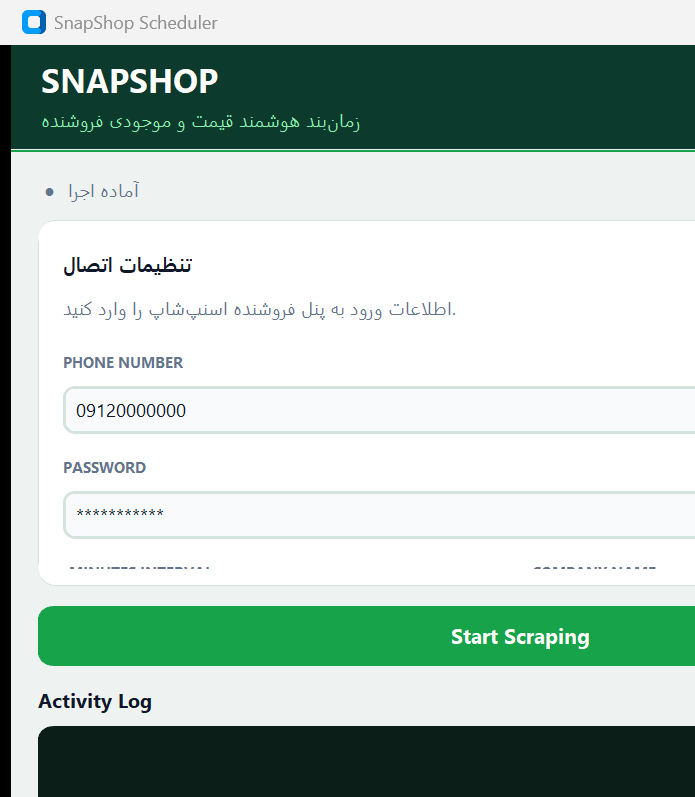
\includegraphics[width=0.88\textwidth]{app_screenshot.png}\\[0.4em]
  {\small\textit{نمایی از رابط کاربری SnapShop Scheduler}}
\end{center}

\vspace{0.6em}

\section{این اپ چه کاری انجام می‌دهد؟}

این برنامه یک \textbf{زمان‌بند خودکار برای مدیریت قیمت و موجودی} فروشنده در فروشگاه اینترنتی \textbf{اسنپ‌شاپ (SnappShop)} است.
با ورود به پنل فروشنده، داده‌های محصولات را استخراج می‌کند، قیمت‌ها را بر اساس قوانین رقابتی (Buybox) تنظیم می‌کند و فایل به‌روزرسانی را دوباره در پنل آپلود می‌کند.

\section{قابلیت‌های اصلی}

\begin{enumerate}[leftmargin=*, itemsep=0.55em]
  \item \textbf{ورود خودکار به پنل فروشنده}\\
  با شماره موبایل و رمز عبور (یا کد تأیید) وارد \lr{seller.snappshop.ir} می‌شود.

  \item \textbf{دانلود فایل موجودی}\\
  از بخش به‌روزرسانی گروهی (\lr{bulk-update}) فایل اکسل محصولات را دانلود می‌کند.

  \item \textbf{اسکرپ Buybox (اختیاری)}\\
  صفحه فروشنده در اسنپ‌شاپ را می‌گردد، قیمت فروشنده دوم و وضعیت بای‌باکس را جمع‌آوری می‌کند تا بتوان قیمت رقابتی تعیین کرد.

  \item \textbf{محاسبه و تنظیم قیمت تخفیف}\\
  برای محصولاتی که فعال‌اند و تخفیف دارند، قیمت بعد از تخفیف را طوری تنظیم می‌کند که نسبت به بای‌باکس رقابتی بماند (مثلاً کمی پایین‌تر از قیمت رقیب).

  \item \textbf{زمان‌بندی دوره‌ای}\\
  همین فرایند را در بازه زمانی مشخص (مثلاً هر ۲۰ دقیقه) به‌صورت خودکار تکرار می‌کند.

  \item \textbf{لاگ زنده}\\
  وضعیت اجرا و خطاها در باکس پایین پنجره نمایش داده می‌شود.
\end{enumerate}

\section{فیلدهای رابط کاربری}

\renewcommand{\arraystretch}{1.4}
\begin{tabular}{>{\raggedright\arraybackslash}p{0.30\textwidth} p{0.60\textwidth}}
\toprule
\textbf{فیلد} & \textbf{توضیح} \\
\midrule
\lr{Phone Number} & شماره موبایل حساب فروشنده اسنپ‌شاپ \\
\lr{Password} & رمز عبور حساب (در صورت غیرفعال کردن «\lr{Use password}»، منتظر ورود دستی کد می‌ماند) \\
\lr{Minutes Interval} & فاصله زمانی تکرار اسکرپ (به دقیقه) \\
\lr{Seller Store URL} & آدرس صفحه فروشنده در اسنپ‌شاپ \\
\lr{Company Name} & نام فروشگاه (مثلاً «چادوک») برای تشخیص فروشنده در بای‌باکس \\
\lr{Skip Buybox scraping} & در صورت فعال بودن، مرحله جمع‌آوری قیمت بای‌باکس رد می‌شود \\
\bottomrule
\end{tabular}

\section{جریان کار به‌صورت خلاصه}

\noindent
\fbox{\parbox{0.94\textwidth}{%
\vspace{0.4em}
\begin{flushleft}
\lr{%
\texttt{Start -> Login to seller panel}\\
\texttt{\phantom{Start} -> Download inventory Excel}\\
\texttt{\phantom{Start} -> (optional) Scrape buybox prices}\\
\texttt{\phantom{Start} -> Filter active discounted products}\\
\texttt{\phantom{Start} -> Update discount start date/time}\\
\texttt{\phantom{Start} -> Calculate competitive price}\\
\texttt{\phantom{Start} -> Build 01.xlsx and upload}\\
\texttt{\phantom{Start} -> Repeat on schedule}%
}
\end{flushleft}
\vspace{0.2em}
}}

\vspace{0.8em}
\noindent
شروع ← ورود به پنل فروشنده ← دانلود اکسل موجودی ← (اختیاری) اسکرپ قیمت بای‌باکس از صفحه عمومی فروشنده ← فیلتر محصولات فعال دارای تخفیف ← به‌روزرسانی تاریخ/ساعت شروع تخفیف ← محاسبه قیمت رقابتی ← ساخت فایل \lr{01.xlsx} و آپلود در پنل ← تکرار طبق بازه زمانی.

\section{خروجی}

نتیجه نهایی معمولاً فایل اکسل \lr{01.xlsx} در پوشه \lr{downloads} است که سپس به‌صورت خودکار در بخش به‌روزرسانی گروهی پنل فروشنده آپلود می‌شود.

\end{document}
